\documentclass[../ai_in_finance]{subfiles}
\usepackage[margin=1in]{geometry}
\usepackage{tikz}
\usetikzlibrary{positioning}
\usepackage{amsmath}
\usepackage{amssymb}
\usepackage{booktabs}
\usepackage{floatrow}
\usepackage{draftwatermark}

\SetWatermarkText{Wulin.Suo@Queensu.ca}
\SetWatermarkScale{1.4}
\SetWatermarkColor{gray!35}
\SetWatermarkAngle{90}
\SetWatermarkHorCenter{0.94\paperwidth}
\SetWatermarkVerCenter{0.5\paperheight}

\usepackage{makeidx}
\makeindex

\begin{document}

\chapter{Market Risk Management}

\section{Introduction}

Every model in this book so far has focused on estimating a quantity of interest: a price, a return, a probability of default, a forecast. Risk management asks a different, complementary question: not ``what do we expect to happen,'' but ``how bad could it get, and how often.'' A portfolio manager who only forecasts expected returns and ignores the distribution of possible losses is flying blind, since the same expected return can come from a smooth, low-volatility strategy or from a strategy that is usually flat but occasionally loses everything.
This chapter introduces the standard toolkit for quantifying and managing that downside for market risk specifically: Value at Risk\index{Value at Risk (VaR)} and Expected Shortfall\index{Expected Shortfall}, maximum drawdown, volatility forecasting, backtesting, liquidity risk, and the model governance and capital adequacy concepts that let a firm and its regulators judge whether it can survive its own worst days.
Chapter 9 develops the parallel toolkit for credit risk, probability of default, loss given default, and credit scoring, since the two risk types, while related, call for genuinely different tools and are large enough topics to deserve their own dedicated treatment.

One worked example runs through most of the chapter: a twenty-day return history for a \$10 million equity portfolio, used to compute and compare parametric, historical, Monte Carlo\index{Monte Carlo simulation}, and GARCH-based risk measures, backtest them, and stress-test the resulting portfolio.

The chapter builds its toolkit in the order a risk desk would actually deploy it. First a taxonomy of risk types (Section~\ref{sec:risk-types}), to establish what is and is not in scope. Then Value at Risk itself (Section~\ref{sec:var}), computed three different ways and then extended to a full portfolio (Section~\ref{sec:matrix-var}), a volatility-adjusted version that updates with Chapter 7's GARCH forecasts (Section~\ref{sec:garch-var}), and the backtesting discipline (Section~\ref{sec:backtesting-var}) that checks whether any of this actually worked out of sample.
Later sections extend the same VaR machinery in three directions: to options positions via the Greeks (Section~\ref{sec:delta-normal}), to hypothetical crises the historical sample never contained (Section~\ref{sec:stress-testing}), and, in Section~\ref{sec:ml-vol-forecast}, to a direct and honest test of whether a more flexible machine learning model can out-forecast GARCH at its own game. Chapter 9 develops the analogous toolkit for credit risk using the same governance and validation philosophy introduced here.

\section{Measuring Market Risk}

This part builds the standard measures in order of increasing honesty about the tail, each worked numerically on the same portfolio.

\subsection{Types of Financial Risk}
\label{sec:risk-types}

Suppose a risk manager reports simply that the fund ``lost money because of risk.'' The statement is true but useless: it does not say whether the loss came from prices moving against a held position, a counterparty failing to pay what it owed, or a position becoming impossible to sell without moving its own price further down, three genuinely different problems that call for three different responses. Financial risk is not a single quantity but a family of related concerns, and confusing one type for another is a common and costly mistake.
Market risk is the risk of loss from movements in prices, rates, or volatilities that a firm is exposed to through the positions it holds; it is the subject of this chapter.
Credit risk is the risk that a counterparty, whether a bond issuer, a loan borrower, or a derivatives counterparty, fails to meet a contractual obligation; Chapter 5 already introduced the pricing consequence of credit risk, and Chapter 9 develops the risk-measurement side of the same problem.
Liquidity risk comes in two related forms: funding liquidity risk, the risk that a firm cannot meet its own cash obligations as they come due, and market liquidity risk, the risk that a position cannot be sold quickly without moving its price significantly against the seller, directly connected to the bid-ask spread\index{bid-ask spread} and market depth concepts of Chapter 3.
Operational risk covers losses from failed internal processes, systems, human error, or external events, including the kind of model risk flagged throughout this book whenever a model's assumptions are quietly violated by a changing environment; Chapter 9 covers a standard capital treatment for it, and Chapter 10 develops the AI methods for detecting and managing it.
Underwriting risk, the risk that claims on policies a firm has written exceed the premiums it collected for them, is the insurer's counterpart to all of the above, and Chapter 11 develops it alongside the reserving and ratemaking machinery it requires.
A single adverse event often touches more than one category at once: a large, sudden market move (market risk) can trigger a wave of defaults among leveraged counterparties (credit risk) precisely when many firms are simultaneously forced to sell into an illiquid market (liquidity risk), which is the contagion dynamic behind the financial crises discussed in Chapter 3.

Table~\ref{tab:risk_taxonomy} summarizes each risk type alongside its standard measurement tool and where in this book that tool is developed, giving a preview of this chapter's structure organized by risk type rather than by technique.

\begin{table}[htbp]
\centering
\begin{lrbox}{\bookmeasuredbox}
\begin{tabular}{p{2.8cm}p{4.6cm}p{6.2cm}}
\toprule
Risk type & Standard measurement tool & Where developed \\
\midrule
Market risk & Value at Risk, Expected Shortfall, maximum drawdown & Sections~\ref{sec:var}--\ref{sec:backtesting-var} of this chapter \\
Credit risk & Probability of default, loss given default, expected loss & Chapter 9 \\
Liquidity risk & Bid-ask spread, liquidity-adjusted VaR & Chapter 3 and later in this chapter \\
Operational risk & Loss distribution approach, scenario analysis, incident-text and anomaly models & Chapter 10, with the regulatory capital charge in Chapter 9 \\
Underwriting risk & Expected loss ratio, combined ratio, chain-ladder reserves & Chapter 11 \\
Systemic risk & Stress testing, contagion modeling & Chapter 3's financial crises discussion, this chapter's stress-testing section, and Chapter 20's network contagion models \\
\bottomrule
\end{tabular}
\end{lrbox}
\ifdim\wd\bookmeasuredbox<0.65\linewidth
\setlength{\bookcapwidth}{0.65\linewidth}
\else
\setlength{\bookcapwidth}{\wd\bookmeasuredbox}
\fi
\floatbox[\capbot]{table}[\bookcapwidth]{
\usebox{\bookmeasuredbox}
}{
\caption{A taxonomy of financial risk types and their standard measurement tools}
\label{tab:risk_taxonomy}
}
\end{table}

\subsection{Value at Risk: Parametric and Historical Methods}
\label{sec:var}

Value at Risk (VaR) answers a specific, deliberately narrow question: over a given holding period and at a given confidence level, what is the loss that will not be exceeded except with some small, specified probability? Formally, the $\alpha$-level VaR of a portfolio is the smallest loss $L$ such that
$$\Pr(\text{Loss} > L) \le 1-\alpha.$$
A 1-day 95\% VaR of \$1 million means that, under the model's assumptions, the portfolio is expected to lose more than \$1 million on only about 5\% of trading days, or roughly one day in twenty.

Table~\ref{tab:portfolio_returns} shows twenty days of returns for a hypothetical \$10 million equity portfolio managed by a firm we will call Meridian Capital Partners.

\begin{table}[htbp]
\centering
\begin{lrbox}{\bookmeasuredbox}
\begin{tabular}{lrrrrrrrrrr}
\toprule
Day & 1 & 2 & 3 & 4 & 5 & 6 & 7 & 8 & 9 & 10 \\
Return & 0.06\% & 0.42\% & -0.27\% & -1.01\% & -0.49\% & -1.13\% & 0.13\% & 1.67\% & -0.53\% & -0.68\% \\
\midrule
Day & 11 & 12 & 13 & 14 & 15 & 16 & 17 & 18 & 19 & 20 \\
Return & 0.65\% & 0.49\% & 0.19\% & -1.06\% & 0.02\% & 0.89\% & -1.55\% & -0.49\% & -2.22\% & -1.49\% \\
\bottomrule
\end{tabular}
\end{lrbox}
\ifdim\wd\bookmeasuredbox<0.65\linewidth
\setlength{\bookcapwidth}{0.65\linewidth}
\else
\setlength{\bookcapwidth}{\wd\bookmeasuredbox}
\fi
\floatbox[\capbot]{table}[\bookcapwidth]{
\usebox{\bookmeasuredbox}
}{
\caption{Twenty days of returns for a \$10 million equity portfolio}
\label{tab:portfolio_returns}
}
\end{table}

The sample mean return is $\bar r = -0.32\%$ and the sample standard deviation is $\hat\sigma = 0.937\%$ (with $n-1=19$ in the denominator, as in every standard-deviation calculation in this book). The parametric (variance-covariance) method assumes returns are normally distributed and computes VaR directly from the mean, standard deviation, and the appropriate normal quantile $z_\alpha$:
\begin{equation*}
\text{VaR}_\alpha = -(\bar r - z_\alpha \hat\sigma) \times V,
\end{equation*}
where $V$ is the portfolio's dollar value. Using $z_{0.95}=1.645$ and $z_{0.99}=2.326$ and $V=\$10{,}000{,}000$,
\begin{equation*}
\text{VaR}_{95\%} = -(-0.0032 - 1.645(0.00937)) \times 10{,}000{,}000 \approx \$186{,}195,
\end{equation*}
\begin{equation*}
\text{VaR}_{99\%} = -(-0.0032 - 2.326(0.00937)) \times 10{,}000{,}000 \approx \$250{,}081.
\end{equation*}
The historical method instead makes no distributional assumption at all: it simply sorts the observed returns and reads the appropriate percentile directly from the data. Sorting the twenty returns in Table~\ref{tab:portfolio_returns} from worst to best, the second-worst return ($-2.22\%$ and $-1.55\%$ are the two worst) corresponds to the 5th percentile of a 20-observation sample, giving
\begin{equation*}
\text{VaR}_{95\%}^{\text{historical}} = -(-0.0155) \times 10{,}000{,}000 = \$155{,}000.
\end{equation*}
The historical and parametric VaR estimates disagree by more than \$30,000 here, which is not a contradiction but a direct illustration of a persistent tension in risk measurement: the parametric method borrows statistical strength from the entire sample and produces a smooth estimate, but it assumes normality, which can be a poor description of returns with heavier tails than a normal distribution predicts, echoing the fat-tails caveat raised in Chapter 7's discussion of GARCH model\index{GARCH model}s. The historical method makes no such assumption, but with only twenty observations, its estimate depends heavily on a single data point (here, the $-1.55\%$ return) and would be considerably more stable with a longer history, typically one to several years of daily data in practice.

\subsubsection*{Portfolio VaR with the Variance-Covariance Matrix}
\label{sec:matrix-var}

The single-return-series version of parametric VaR above is a special case of a more general matrix formula that extends naturally to a portfolio of several assets. Recall the two-asset covariance matrix from Chapter 2's worked AssetA/AssetB example,
\begin{equation*}
\Sigma = \begin{pmatrix} 0.000414 & -0.000198 \\ -0.000198 & 0.000118 \end{pmatrix},
\end{equation*}
computed there from the two assets' daily returns, and the equal weights $w = (0.5, 0.5)$ used throughout that chapter. The portfolio's return variance is $w^\top \Sigma w$, the formula Chapter 2 verified numerically, and the parametric VaR of a portfolio worth $V$ dollars, assuming a zero mean return (a common simplification in practice, since a one-day expected return is typically negligible relative to one-day volatility), is
\begin{equation*}
\text{VaR}_\alpha \approx z_\alpha \sqrt{w^\top \Sigma w}\; V.
\end{equation*}
Applying this to a hypothetical \$2 million position split evenly between AssetA and AssetB, $\sqrt{w^\top \Sigma w} \approx 0.583\%$ (matching the portfolio volatility computed in Chapter 2), so
\begin{equation*}
\text{VaR}_{95\%} \approx 1.645(0.00583)(2{,}000{,}000) \approx \$19{,}182,
\end{equation*}
\begin{equation*}
\text{VaR}_{99\%} \approx 2.326(0.00583)(2{,}000{,}000) \approx \$27{,}130.
\end{equation*}
This matrix formulation is what actually scales to real trading books, which routinely hold hundreds or thousands of positions: rather than tracking a single blended portfolio-return series, a risk system maintains the full covariance matrix $\Sigma$ across every position and recomputes $w^\top \Sigma w$ whenever positions change, the same computational pattern Chapter 2 introduced for a portfolio of arbitrary size using \texttt{weights @ cov\_matrix.values @ weights}.

\subsubsection*{Component VaR: Decomposing Portfolio Risk by Position}\index{Component VaR}

A portfolio-level VaR figure answers ``how much risk does the whole book have,'' but a risk manager allocating limits across desks, or a portfolio manager deciding which position to trim first, needs the complementary question: how much of that risk does each individual position actually contribute? Component VaR answers this by decomposing total portfolio variance into a sum of per-asset contributions, using the same covariance matrix already in hand,
\begin{equation*}
\text{Component Var}_i = w_i (\Sigma w)_i, \qquad \sum_i \text{Component Var}_i = w^\top \Sigma w,
\end{equation*}
so that each asset's fractional share of total portfolio variance, $\text{Component Var}_i / (w^\top\Sigma w)$, scales the total portfolio VaR into a per-asset Component VaR that sums exactly back to the whole. Applying this to Section~\ref{sec:matrix-var}'s two-asset position, $\Sigma w = (0.000108, -0.00004)$, so
\begin{align*}
\text{Component Var}_A &= 0.5(0.000108) = 0.000054, \\
\text{Component Var}_B &= 0.5(-0.00004) = -0.00002,
\end{align*}
summing to the portfolio variance of $0.000034$ exactly as required. Scaling these fractions ($1.588$ and $-0.588$) by the total $\text{VaR}_{95\%}$ of \$19,182 gives
\begin{equation*}
\text{Component VaR}_A \approx \$30{,}468, \qquad \text{Component VaR}_B \approx -\$11{,}285,
\end{equation*}
which sum back to the \$19,182 total, exactly as the decomposition guarantees. AssetB's component is \emph{negative}, even though AssetB has positive standalone volatility on its own. Its strongly negative correlation with AssetA (Section~\ref{sec:stress-testing} computes it as $\rho\approx-0.896$) makes it a diversifier within this specific portfolio: adding more of AssetB, holding AssetA fixed, would actually \emph{reduce} total portfolio risk, not add to it. That is a fact the standalone volatility figures for AssetA and AssetB alone could never reveal.
This is precisely why risk limits at a real trading firm are typically set and monitored using component or marginal VaR rather than standalone position size or standalone volatility: a position's true risk contribution depends on how it interacts with everything else already in the book, not on how risky it looks in isolation.

\subsection{Expected Shortfall: Going Beyond VaR}

VaR has a well-known conceptual weakness: it answers ``how much can I lose with 95\% confidence,'' but says nothing about how bad the remaining 5\% of outcomes actually are. Two portfolios can have identical VaR while one has a slightly worse tail and the other has a catastrophically worse one. Expected Shortfall (ES), also called Conditional VaR, addresses this directly by averaging the losses in the tail beyond VaR rather than simply reporting its boundary:
\begin{equation*}
\text{ES}_\alpha = \mathbb{E}[\text{Loss} \mid \text{Loss} > \text{VaR}_\alpha].
\end{equation*}
For the historical method applied to Table~\ref{tab:portfolio_returns}, the two worst returns ($-2.22\%$ and $-1.55\%$) are the ones at or beyond the 95\% VaR threshold, so
\begin{equation*}
\text{ES}_{95\%}^{\text{historical}} = -\frac{(-0.0222) + (-0.0155)}{2} \times 10{,}000{,}000 = \$188{,}500.
\end{equation*}
The parametric Expected Shortfall under normality has a closed-form expression involving the standard normal density $\phi(\cdot)$,
\begin{equation*}
\text{ES}_\alpha = \left(\hat\sigma \frac{\phi(z_\alpha)}{1-\alpha} - \bar r\right) \times V,
\end{equation*}
which for $\alpha=95\%$ gives $\text{ES}_{95\%} \approx \$225{,}366$, noticeably larger than the parametric VaR$_{95\%}$ of \$186,195, exactly as it should be, since ES averages over the full tail rather than reporting only its edge.
Because ES is a coherent risk measure\index{Coherent Risk Measure} in a precise mathematical sense that VaR is not (it satisfies a subadditivity property guaranteeing that diversification can never increase measured risk, which VaR can occasionally violate in pathological cases), banking regulators have shifted market-risk capital requirements from VaR toward Expected Shortfall in recent years, a change explored further in this chapter's discussion of regulatory capital. Figure~\ref{fig:var_es_tail} shows why the two measures differ: VaR marks only the boundary of the shaded loss tail, while ES averages over the entire tail beyond it.

\begin{figure}[htbp]
\centering
\begin{lrbox}{\bookmeasuredbox}
    % scale + transform shape, as in Figures 6.7 and 6.10: the curve, the shaded
    % tail, and both annotations shrink together, so nothing collides.
    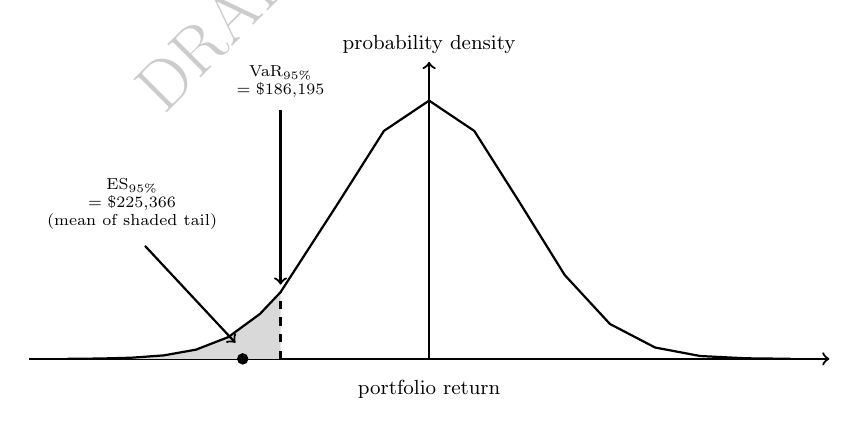
\begin{tikzpicture}[thick,scale=0.82,
        every node/.append style={transform shape}]
        \draw[->] (-6.2,0) -- (6.2,0);
        \draw[->] (0,0) -- (0,4.6) node[above,font=\small] {probability density};
        \node[below,font=\small] at (0,-0.2) {portfolio return};
        \fill[gray!30] (-5.60,0.001) -- (-5.10,0.005) -- (-4.61,0.018) -- (-4.11,0.054) -- (-3.61,0.143) -- (-3.11,0.337) -- (-2.62,0.696) -- (-2.30,1.034) -- (-2.30,0) -- (-5.60,0) -- cycle;
        \draw[solid] (-5.60,0.001) -- (-5.10,0.005) -- (-4.61,0.018) -- (-4.11,0.054) -- (-3.61,0.143) -- (-3.11,0.337) -- (-2.62,0.696) -- (-2.30,1.034) -- (-1.40,2.426) -- (-0.70,3.530) -- (0.00,4.000) -- (0.70,3.530) -- (1.40,2.426) -- (2.10,1.299) -- (2.80,0.541) -- (3.50,0.176) -- (4.20,0.044) -- (4.90,0.009) -- (5.60,0.001);
        \draw[dashed] (-2.30,0) -- (-2.30,1.034);
        \node[align=center,font=\scriptsize] at (-2.30,4.3) {$\text{VaR}_{95\%}$\\$=\$186{,}195$};
        \draw[->] (-2.30,3.85) -- (-2.30,1.15);
        \filldraw (-2.887,0) circle (2pt);
        \node[align=center,font=\scriptsize] at (-4.6,2.4) {$\text{ES}_{95\%}$\\$=\$225{,}366$\\(mean of shaded tail)};
        \draw[->] (-4.4,1.75) -- (-3.0,0.25);
    \end{tikzpicture}
\end{lrbox}
\ifdim\wd\bookmeasuredbox<0.65\linewidth
\setlength{\bookcapwidth}{0.65\linewidth}
\else
\setlength{\bookcapwidth}{\wd\bookmeasuredbox}
\fi
\ffigbox[\bookcapwidth]{
\usebox{\bookmeasuredbox}
}{
    \caption{The parametric VaR and Expected Shortfall of Table~\ref{tab:portfolio_returns}'s portfolio, illustrated against the assumed normal return distribution}
    \label{fig:var_es_tail}
}
\end{figure}

\subsection{Maximum Drawdown: A Path-Dependent Risk Measure}\index{Maximum drawdown}
\label{sec:max-drawdown}

Value at Risk and Expected Shortfall both summarize the distribution of possible one-day losses, but neither says anything about a different, equally practical question: how much value would an investor holding this portfolio actually have seen erode from its own peak over an extended period, not just on any single day? Maximum drawdown answers this. Given a portfolio value path $V_0, V_1, \ldots, V_T$, the drawdown at time $t$ is the percentage decline from the running peak up to and including that point,
\begin{equation*}
\text{Drawdown}_t = \frac{\max_{0 \le s \le t} V_s - V_t}{\max_{0 \le s \le t} V_s} \ge 0,
\end{equation*}
and the maximum drawdown over the full path is simply the worst (largest) drawdown observed anywhere along it, $\text{MDD} = \max_{0\le t \le T} \text{Drawdown}_t$. Unlike VaR and Expected Shortfall, which depend only on the distribution of individual returns and not on their order, maximum drawdown is inherently path-dependent. Shuffling the same twenty daily returns into a different sequence would generally change the maximum drawdown, even though every VaR and Expected Shortfall figure computed from them would be identical. Both the peak against which decline is measured and the trough that realizes it depend on exactly \emph{when}, not just how large, the losses occur.

Applying this to the cumulative value path implied by Table~\ref{tab:portfolio_returns}'s twenty daily returns, starting from the portfolio's initial \$10,000,000, the running peak of \$10,048,025 is reached after Day 2, following two small positive returns, and the portfolio's value never again exceeds that peak for the remainder of the sample; its lowest point, \$9,371,210, occurs at the very end, Day 20, after four consecutive negative returns on Days 17 through 20. The maximum drawdown is therefore
\begin{equation*}
\text{MDD} = \frac{10{,}048{,}025 - 9{,}371{,}210}{10{,}048{,}025} \approx 6.74\%, \qquad \text{a peak-to-trough decline of } \$676{,}815.
\end{equation*}
This is a materially different, and arguably more decision-relevant, number than the portfolio's cumulative return over the full twenty days, only $-6.29\%$. The extra $0.45$ percentage points of drawdown reflect the fact that the portfolio was briefly \emph{up} \$48,025 before its losses began. An investor who happened to hold the position from Day 2 onward therefore experienced a larger peak-to-trough decline than a naive start-to-end comparison alone would reveal.
This is the sense in which maximum drawdown captures something the chapter's daily VaR figures cannot. A portfolio whose losses on every individual day comfortably clear a well-calibrated 95\% VaR threshold can still suffer a large, sustained drawdown if enough of those daily losses occur consecutively rather than being offset by intervening gains, the pattern in this example's final four days.

Maximum drawdown is used throughout this book wherever a full return path, not just a single day's distribution, is the natural object of interest. Chapter 13 uses it directly, alongside the Sharpe ratio and hit rate, to evaluate a backtested trading strategy's worst peak-to-trough decline. Asset managers and hedge funds routinely report it as a standard risk statistic, precisely because, unlike VaR, it requires no distributional assumption at all, only a value path. It is also immediately interpretable to an investor asking, in plain language, ``how much could I have lost had I been unlucky enough to enter at the worst possible time.''
Its main limitation mirrors that same simplicity. A single realized maximum drawdown is one historical observation of a path-dependent statistic, not an estimate of a full distribution the way VaR or Expected Shortfall are. Comparing two strategies' historical maximum drawdowns therefore says less about their future worst-case risk than comparing their VaR or Expected Shortfall figures would.

\subsection{Monte Carlo Simulation for Risk Measurement}

A third approach, Monte Carlo simulation, sits between the parametric and historical methods: it assumes a distributional model, as the parametric method does, but instead of relying on a closed-form formula, it simulates a very large number of hypothetical return scenarios from that model and reads VaR and ES directly off the simulated distribution, exactly as the historical method reads them off the observed one.
Simulating 100,000 draws from a normal distribution with the same mean and standard deviation as Table~\ref{tab:portfolio_returns} ($\bar r=-0.32\%$, $\hat\sigma=0.937\%$) gives $\text{VaR}_{95\%} \approx \$187{,}460$, $\text{VaR}_{99\%} \approx \$251{,}690$, and $\text{ES}_{95\%} \approx \$226{,}378$. All are close to the parametric formulas above, as they should be: with enough simulated draws, Monte Carlo VaR converges to the exact parametric answer whenever the underlying model is one for which a closed form exists at all.

The method's real value emerges precisely when no such closed form is available, for example a portfolio containing options (whose payoffs are nonlinear in the underlying price, a case Section~\ref{sec:delta-normal} returns to directly) or a model with fat tails, jumps, or time-varying volatility of the kind introduced in Chapter 7's GARCH models. In those cases, Monte Carlo simulation remains straightforward, simulate many paths under the more realistic model and read off the empirical percentile, while a closed-form parametric formula either does not exist or requires a much more complex derivation.

\subsubsection*{Volatility-Adjusted VaR: Connecting GARCH Forecasts to Risk Measurement}\index{Volatility-Adjusted VaR}
\label{sec:garch-var}

Every VaR method above shares a hidden assumption: each uses a single volatility estimate, computed once from a fixed historical window, and holds it fixed. Chapter 7's GARCH(1,1) model suggests a more responsive alternative, since volatility itself clusters and evolves: rather than a static historical standard deviation, a VaR estimate can be updated every day using the GARCH model's own one-step-ahead variance forecast, an approach widely used in practice and sometimes called volatility-adjusted or ``GARCH VaR.''

Recall Chapter 7's GARCH(1,1) recursion applied to Chapter 2's four AssetA returns ($\omega=0.00002$, $\alpha=0.10$, $\beta=0.85$): the one-step-ahead forecast volatility was $1.95\%$ immediately before the large $+2.97\%$ return at $t=3$, and rose to $2.08\%$ immediately after it. Applying the same parametric VaR formula as Section~\ref{sec:var}, but with each of these two GARCH-forecast volatilities in place of a static historical standard deviation, to a hypothetical \$10 million position gives
\begin{align*}
\text{VaR}_{95\%}^{\text{pre-shock}} &= 1.645(0.0195)(10{,}000{,}000) \approx \$320{,}775, \\
\text{VaR}_{95\%}^{\text{post-shock}} &= 1.645(0.0208)(10{,}000{,}000) \approx \$342{,}160,
\end{align*}
an increase of about $6.7\%$ in a single day, purely from the GARCH model's own updated variance forecast, with no new position taken and no change to the portfolio itself. A VaR model relying on a rolling historical-window standard deviation instead would still be averaging in several of the calmer, pre-shock returns and would understate the position's risk for as long as those calmer observations remain in the averaging window, precisely the lag GARCH's recursive weighting is designed to avoid. This is the volatility-clustering-aware risk measurement Chapter 7 flagged GARCH as being useful for, applied directly to the VaR machinery of this chapter.

\subsubsection*{Filtered Historical Simulation: Combining the Two Methods}\index{Filtered Historical Simulation}

The historical method (Section~\ref{sec:var}) and the GARCH-based method just introduced solve two different problems well: the historical method captures the actual shape of the return distribution, its skew and fat tails, without imposing a normal-distribution assumption, while GARCH captures how much that distribution's width is currently elevated or depressed relative to its long-run average.
Filtered historical simulation combines both strengths in a single procedure. Each historical return $r_t$ is first standardized by the GARCH volatility estimate prevailing on that same day, $z_t = r_t/\sigma_t$, producing a series of standardized residuals that should be roughly free of volatility clustering if the GARCH model is well specified; VaR is then read off the appropriate percentile of this standardized series, and rescaled by \emph{today's} GARCH forecast volatility rather than whatever volatility happened to prevail on the day each historical return was originally observed.

Applying this logic to the two GARCH forecasts already computed, $\sigma_3=1.95\%$ (pre-shock) and $\sigma_4=2.08\%$ (post-shock): a large historical return observed during the calmer $t=3$ regime, divided by that day's own small $\sigma_t$, contributes a large standardized residual, exactly as it should, since that return was unusually large \emph{relative to its own volatility regime}, not just in absolute terms.

Chapter 2's AssetA series supplies exactly such an observation. The $+2.97\%$ return arrived while $\sigma_3 = 1.95\%$ prevailed, the calmest forecast in the whole recursion, so its standardized residual is
\begin{equation*}
z_3 = \frac{0.0297}{0.0195} = 1.523,
\end{equation*}
and rescaling that residual by the post-shock forecast $\sigma_4 = 2.08\%$ gives a hypothetical return for today's conditions of $1.523 \times 0.0208 = 3.17\%$. Plain historical simulation would have reused the $2.97\%$ figure unchanged, understating the move by about twenty basis points for no reason other than that the return happened to be observed in a calmer volatility regime than the one now prevailing.

That is the general procedure: rescaling a standardized residual by today's forecast volatility, whatever it currently is, produces a properly scaled hypothetical return for today's actual conditions, avoiding both the plain historical method's problem (treating every day's return as if it occurred under today's volatility) and the plain parametric method's problem (imposing normality on a shape that raw historical data might contradict). Filtered historical simulation is the kind of practical middle ground large trading desks use in production VaR systems, requiring the same GARCH machinery already developed above, applied across an entire historical return series rather than to a single day's forecast.

\section{Validating and Extending the Measures}

A risk number nobody has tested is a decoration; this part checks the measures against realized losses and extends them where the simple versions break.

\subsection{Backtesting Value at Risk Models}
\label{sec:backtesting-var}

A VaR model is only useful if it is actually calibrated\index{calibration} correctly, and the standard way to check this is backtesting: comparing how often realized losses actually exceeded the model's VaR threshold (an ``exception'') against how often the model itself predicted an exception should occur. A well-calibrated 95\% VaR model should produce an exception on roughly 5\% of days, no more and, just as importantly, no fewer, since a model that is never exceeded is not necessarily good news; it may simply be too conservative, tying up capital that could otherwise be deployed productively.

Applying the parametric $95\%$ VaR threshold from Section~\ref{sec:var} (a daily return of $-1.862\%$, equivalent to the \$186,195 VaR figure) to the twenty returns in Table~\ref{tab:portfolio_returns}, exactly one return, the $-2.22\%$ observation, falls below the threshold, for an observed exception rate of $1/20 = 5\%$, matching the model's target almost exactly. Applying the parametric $99\%$ threshold (a return of $-2.501\%$) produces zero exceptions, consistent with an expected count of $0.01 \times 20 = 0.2$ exceptions, since zero is the natural outcome when the expected count is already well below one.

Kupiec's proportion-of-failures (POF) test\index{Kupiec's proportion-of-failures (POF) test} formalizes this comparison, testing the null hypothesis that the model's true exception rate equals its target $p$ against a likelihood-ratio statistic,
\begin{equation*}
LR_{\text{POF}} = -2\ln\left[\frac{(1-p)^{n-x}p^x}{(1-x/n)^{n-x}(x/n)^x}\right],
\end{equation*}
which is compared against a chi-squared distribution with one degree of freedom (critical value $3.841$ at the conventional 95\% test level) under the null. For the twenty-day sample above, with $p=0.05$, $n=20$, and $x=1$ exception, the observed rate $x/n=1/20=0.05$ exactly equals the target $p$, so the numerator and denominator are identical and $LR_{\text{POF}}=0$, nowhere close to rejecting the null.

This looks like a perfect endorsement of the model, but it is really a demonstration of the same small-sample caution raised throughout this book: a single additional bad day would move the observed rate to $2/20=10\%$, and even that doubled exception rate would not, by itself, generate enough evidence at only twenty observations to reliably distinguish a well-calibrated model from a miscalibrated one. Kupiec's test, and the Basel traffic-light framework built on the same underlying logic, require a considerably longer history, typically the full one-year, 250-observation window described below, before they have any real statistical power, exactly as Chapter 7's Dickey-Fuller test did: a test can be constructed and interpreted correctly and still lack the power to detect a real problem on a short sample.

Backtesting failures are taken seriously by regulators: under the Basel framework\index{Basel Accords}, a bank whose internal VaR model produces too many exceptions in a rolling one-year window can be required to hold additional regulatory capital, using a multiplier applied directly to the reported VaR figure, which creates a direct financial incentive for banks to calibrate their risk models honestly rather than reporting an artificially low VaR to reduce capital requirements.

\subsubsection*{The Basel Traffic-Light Backtesting Framework}\index{Basel Traffic-Light Backtesting Framework}

Basel formalizes this backtesting logic into a three-zone ``traffic light'' system, based on the number of VaR exceptions observed over a rolling 250-trading-day window at the 99\% confidence level, where $0.01 \times 250 = 2.5$ exceptions are expected on average if the model is correctly calibrated. Zero to four exceptions fall in the green zone, requiring no action beyond continued monitoring and leaving the baseline capital multiplier of 3 unchanged.
Five to nine exceptions fall in the yellow zone, triggering closer supervisory scrutiny and an increased capital multiplier that scales up within the zone; and ten or more exceptions fall in the red zone, where the model is presumed flawed and the multiplier rises to its maximum regulatory level of 4.

This framework only works as intended over its full 250-day design window, which is worth underscoring using this chapter's own toy example: Table~\ref{tab:portfolio_returns}'s twenty-day, one-exception sample cannot be classified into a zone at all, since the traffic-light thresholds are calibrated to 250 observations, not twenty.
Naively extrapolating the observed rate ($1/20=5\%$) to a full year would suggest roughly twelve or thirteen exceptions, which would fall well into the red zone. But doing so would repeat the small-sample overreach Section~\ref{sec:backtesting-var} just cautioned against. Twenty days is nowhere near enough data to support that extrapolation, and the traffic-light system is explicitly designed to be read only once a full 250-day window has actually been observed, not inferred from a short sample no matter how suggestive it looks.

\subsubsection*{Backtesting Expected Shortfall}\index{Backtesting Expected Shortfall}

The regulatory shift from VaR to Expected Shortfall raises a genuine methodological complication: VaR backtesting reduces to counting exceptions, a simple binary event (did the loss exceed the threshold or not) that Kupiec's test and the traffic-light framework both build on directly, but ES is an average of losses \emph{within} the tail, so a single exceedance day does not, by itself, say whether the model's ES forecast was too high, too low, or about right.

A common practical approach compares the \emph{realized} loss on each exception day to the model's ES forecast for that same day, averaged across however many exceptions have occurred. Table~\ref{tab:portfolio_returns}'s single 95\% exception, the $-2.22\%$ return, realizes a loss of $0.0222 \times 10{,}000{,}000 = \$222{,}000$ against the parametric $\text{ES}_{95\%}$ forecast of \$225,366 computed earlier, a ratio of about $0.985$, suggesting the forecast was, if anything, very slightly conservative on this one occurrence.

A single exception is obviously far too little evidence to validate an ES model on its own, but the underlying comparison, average realized loss on exception days against the model's own ES forecast for those days, is how a real trading desk accumulates the longer track record needed to judge whether its ES model is well calibrated, not merely whether its VaR threshold is crossed the right number of times.

\subsubsection*{From Daily VaR to Economic Capital: Time Scaling and Its Limits}\index{Economic capital}
\label{sec:econ-capital}

Every VaR figure computed above answers a specific one-day question, but two further, related questions arise directly from it in practice: how much capital should be held against a longer regulatory horizon, and how much capital should the institution as a whole hold, over a full year, to survive a genuinely severe loss with high confidence? Both questions build on the same daily VaR already computed, using a time-scaling shortcut and a much higher confidence level, respectively.

Basel's market-risk capital framework historically scaled a bank's daily VaR up to a 10-day regulatory horizon using the square-root-of-time rule\index{square-root-of-time rule},
\begin{equation*}
\text{VaR}_T \approx \text{VaR}_1 \sqrt{T},
\end{equation*}
which holds exactly when daily returns are independent and identically distributed, since the variance of a sum of $T$ independent, identically distributed daily returns is exactly $T$ times the one-day variance. Applying this to the parametric 99\% VaR of \$250,081 computed in Section~\ref{sec:var} gives a 10-day regulatory VaR of $250{,}081\sqrt{10}\approx\$790{,}824$, computed once from the same daily figure rather than requiring an entirely separate 10-day model.

The independence assumption behind this shortcut, however, is the assumption Chapter 7 spent an entire chapter warning against: real daily returns are rarely perfectly independent, and even a modest positive autocorrelation meaningfully changes how fast multi-day risk actually grows. If daily returns instead followed an AR(1) process with a modest autocorrelation of $\phi=0.10$ (much weaker than the $\phi=0.71$ Chapter 7 estimated for interest-rate deviations, but still a realistic magnitude for daily equity returns), the variance of a $T$-day cumulative return is
\begin{equation*}
\text{Var}\left(\sum_{t=1}^T r_t\right) = T\sigma^2 + 2\sigma^2\sum_{k=1}^{T-1}(T-k)\phi^k,
\end{equation*}
which for $T=10$ gives a true 10-day volatility about $9.4\%$ higher than the square-root-of-time rule assumes, and correspondingly a true 10-day 99\% VaR of about \$865,413 rather than \$790,824: the square-root-of-time shortcut, applied to autocorrelated returns, quietly understates the regulatory capital a bank should actually hold, in the direction that matters (understating risk, not overstating it).

Economic capital extends this same time-scaling logic one step further, from a 10-day regulatory horizon to a full one-year horizon calibrated to a much higher confidence level, typically 99.9\% or higher, chosen to be consistent with the default probability of the credit rating (commonly single-A or double-A) a bank wants its own solvency to reflect; Chapter 9 develops the analogous calculation directly for credit portfolios using the Vasicek model.
Unlike the regulatory VaR multiplier in Section~\ref{sec:backtesting-var}, which is a supervisory capital charge computed from a specific, prescribed methodology, economic capital is a bank's own internal estimate of how much capital its entire risk-taking business genuinely needs to survive a severe, low-probability year. It is used as much for internal capital allocation and performance measurement as for regulatory compliance: a desk generating a given return on a smaller economic-capital charge is, all else equal, using the firm's scarce capital more efficiently.

\subsection{Liquidity Risk and Liquidity-Adjusted VaR}

Every VaR calculation so far has implicitly assumed that a position can be liquidated at the current market price, but Chapter 3 already established that this is not quite right: selling a position, especially a large or illiquid one, costs at least half the bid-ask spread relative to the mid price, and a large enough order can walk through several levels of the order book at a progressively worse price, just as in Chapter 3's limit-order-book example. Liquidity-adjusted VaR (LVaR) incorporates this directly by adding an estimated liquidation cost to the standard VaR figure,
\begin{equation*}
\text{LVaR}_\alpha = \text{VaR}_\alpha + \frac{1}{2}\,(\text{spread}) \times V,
\end{equation*}
where the spread is expressed as a fraction of position value and the factor of one-half reflects the cost of crossing from the mid price to the relevant side of the quote, the same logic used to compute the round-trip trading cost in Chapter 3. Applying this to the \$2 million two-asset position from Section~\ref{sec:matrix-var}, assuming an average bid-ask spread of 30 basis points, the liquidity cost adjustment is
\begin{equation*}
\frac{1}{2}(0.0030)(2{,}000{,}000) = \$3{,}000, \qquad \text{LVaR}_{95\%} = 19{,}182 + 3{,}000 = \$22{,}182,
\end{equation*}
an increase of roughly 16\% over the standard parametric VaR of \$19,182.
This adjustment matters most precisely in the conditions where it is most often ignored. During a market-wide liquidity crunch, bid-ask spreads themselves widen sharply; recall from Chapter 3 that spreads compensate market makers for inventory risk and adverse selection, both of which increase during stressed markets. The true cost of liquidating a position exactly when a firm most needs to reduce risk can therefore be far higher than a liquidity adjustment calibrated on calm-market spreads would suggest, another instance of the procyclicality problem discussed later in this chapter.

Market liquidity risk, the focus above, is distinct from funding liquidity risk, the risk that a firm cannot meet its own near-term cash obligations, and Basel III addresses the latter directly with the Liquidity Coverage Ratio (LCR)\index{Liquidity Coverage Ratio (LCR)},
\begin{equation*}
\text{LCR} = \frac{\text{High-Quality Liquid Assets}}{\text{Total Net Cash Outflows over 30 days}} \ge 100\%,
\end{equation*}
which requires a bank to hold enough genuinely liquid assets (cash and high-grade government bonds, broadly) to survive 30 days of a specified stress scenario without needing to raise new funding. A bank with \$50 million in high-quality liquid assets and projected net cash outflows of \$40 million over a 30-day stress scenario has $\text{LCR} = 50/40 = 125\%$, comfortably above the regulatory minimum.
The LCR is best understood as a funding-side complement to the market-side liquidity-adjusted VaR above. Liquidity-adjusted VaR asks how much a specific position would cost to sell; the LCR asks whether the firm as a whole has enough liquid resources on hand to avoid being a forced seller of anything at all during a period of stress. That is precisely the scenario, forced selling into an already-stressed and illiquid market, that turned market liquidity risk into a systemic problem during the 2008 crisis discussed later in this chapter.

Basel III pairs the LCR with a second, longer-horizon ratio, the Net Stable Funding Ratio (NSFR)\index{Net Stable Funding Ratio (NSFR)},
\begin{equation*}
\text{NSFR} = \frac{\text{Available Stable Funding}}{\text{Required Stable Funding}} \ge 100\%,
\end{equation*}
which asks essentially the same question as the LCR, does the bank have enough stable funding on hand, but over a one-year horizon rather than 30 days, and weighted toward the structural mismatch between how long a bank's assets take to mature (loans, often years) and how quickly its liabilities could be withdrawn (deposits, often on demand).
Available stable funding weights a bank's capital and liabilities by how reliably they will still be there in a year (retail deposits are weighted as more stable than short-term wholesale borrowing, for instance), while required stable funding weights its assets by how long they are locked up (a long-dated loan requires more stable funding backing it than an overnight reverse repo).
Where the LCR addresses a sudden, short-term liquidity run, the NSFR addresses the slower-moving risk of a bank funding long-term assets with short-term, flighty liabilities, the maturity-transformation mismatch that turned a funding problem into a solvency problem for several institutions during the 2008 crisis once wholesale funding markets froze.

\subsubsection*{VaR for Nonlinear Portfolios: The Delta-Normal Approximation and Its Limits}\index{Delta-Normal Approximation}
\label{sec:delta-normal}

Every VaR calculation so far has assumed a linear portfolio: one whose value moves in direct, constant proportion to the underlying risk factor. A portfolio containing options violates this assumption, and Chapter 5's Greeks give the vocabulary to see exactly how.

Consider a market maker short 1,000 of the one-year, \$50-strike calls priced in Chapter 5 ($S_0=K=\$50$, $r=4\%$, $\sigma=30\%$, $C_0\approx\$6.88$, $\Delta=0.6115$, $\Gamma=0.0255$). The delta-normal method approximates the position's one-day loss using only delta, treating the option price as locally linear in the stock price.
Converting the annual volatility to a daily figure the standard way, $\sigma_{\text{daily}} = 0.30/\sqrt{252} \approx 1.90\%$, the position's delta-implied one-day dollar standard deviation is
\begin{equation*}
\Delta \times S_0 \times \sigma_{\text{daily}} \times 1{,}000 = 0.6115 \times 50 \times 0.0190 \times 1{,}000 \approx \$577.85,
\end{equation*}
giving $\text{VaR}_{95\%}^{\text{delta-normal}} \approx 1.645(577.85) \approx \$950.56$ and $\text{VaR}_{99\%}^{\text{delta-normal}} \approx 2.326(577.85) \approx \$1{,}344.08$.

Full revaluation instead reprices the same option with the same Black-Scholes-Merton formula at a stressed stock price, holding strike, rate, volatility, and time to maturity fixed (a simplification that ignores one day of time decay, isolating the delta and gamma effect this example is meant to illustrate).
The worst case for a short call is the stock rising, so at the 95\% stressed price $S_0(1+z_{0.95}\sigma_{\text{daily}}) \approx \$51.55$, the same option reprices to \$7.86, a position loss of \$980.79, about $3.2\%$ \emph{more} than the delta-normal estimate. At the more extreme 99\% stressed price of \$52.20, the option reprices to \$8.28, a loss of \$1,403.99, now about $4.5\%$ more than delta-normal predicted.

A delta-gamma approximation\index{Delta-Gamma Approximation} closes most of this gap without requiring a full revaluation, by adding a quadratic correction term built directly from the same gamma already computed in Chapter 5,
\begin{equation*}
\Delta P \approx \left(\Delta \, \Delta S + \tfrac{1}{2}\Gamma \, \Delta S^2\right) \times n_{\text{contracts}}.
\end{equation*}
With $\Delta S_{95} = S_0 z_{0.95}\sigma_{\text{daily}} \approx \$1.554$ and $\Delta S_{99} \approx \$2.198$, this gives delta-gamma losses of
\begin{align*}
1{,}000\left(0.6115(1.554) + \tfrac{1}{2}(0.0255)(1.554)^2\right) &\approx \$981.43, \\
1{,}000\left(0.6115(2.198) + \tfrac{1}{2}(0.0255)(2.198)^2\right) &\approx \$1{,}405.79,
\end{align*}
within a few cents of the full-revaluation figures of \$980.79 and \$1,403.99, compared to delta-normal's \$950.56 and \$1,344.08. The quadratic term costs only one extra number, gamma, already available from Chapter 5's Greeks, and recovers nearly all of the accuracy a full repricing would have provided, which is why delta-gamma VaR, rather than delta-normal alone or full revaluation of every position, is the standard compromise used in practice for portfolios with too many options to reprice individually at every stressed scenario.
This growing gap is exactly gamma's effect: delta describes the option's slope at the current stock price, but a genuinely large move travels far enough along the price-value curve that the slope itself has changed by the time the move is complete, and gamma measures precisely that curvature.
The delta-normal method is a reasonable, cheap approximation for small moves or a portfolio with little gamma exposure relative to its size, but it systematically understates risk for a portfolio with meaningful gamma, understating it more severely the larger and more extreme the move being measured, exactly why the 99\% gap above is proportionally wider than the 95\% gap. A trading desk with substantial options exposure therefore typically supplements delta-normal VaR with full revaluation, or with a second-order delta-gamma approximation that adds a quadratic correction term, precisely to correct for this shortfall.

\subsection{Sensitivity-Based Risk Limits}\index{Sensitivity-based risk limits}
\label{sec:sensitivity-limits}

A desk can sit comfortably inside every VaR limit it has been given and still be carrying the position that ends its year. The reason is structural rather than a failure of calibration: VaR compresses an entire book into a single number, and that compression is exactly what hides where the risk actually sits. Two desks reporting the same \$300,000 daily VaR can hold portfolios with nothing in common, one of them perfectly hedged against the move that is about to happen and the other pointed directly into it.

Practitioners therefore run sensitivities alongside VaR, never instead of it. A sensitivity answers a different and much narrower question than VaR does: not ``how bad could tomorrow be, all things considered,'' but ``if this one risk factor moves by one unit, and nothing else changes, how much money do we make or lose?'' The answers are unglamorous, linear, and immediately actionable, which is precisely why the trading floor lives on them.

\subsubsection*{The Greeks as Limits in Their Own Right}

Chapter 5 computed delta, gamma, vega, and theta for the option this chapter has been using, and Section~\ref{sec:delta-normal} then drew on the first two of them, but only as ingredients in a VaR approximation. On a real derivatives desk each is a limit in its own right, monitored and enforced independently of any VaR number. Return to that section's position, a market maker short 1,000 of Chapter 5's one-year \$50-strike calls ($S_0=K=\$50$, $r=4\%$, $\sigma=30\%$), and read the whole set as a risk report rather than as pricing output. Table~\ref{tab:greek_limits} collects them, scaled to the position and joined by rho, the one Greek Chapter 5 did not compute.

\begin{table}[htbp]
\centering
\begin{lrbox}{\bookmeasuredbox}
\begin{tabular}{p{2.0cm}p{4.6cm}rrr}
\toprule
Greek & Measures exposure to & Position & Limit & Utilization \\
\midrule
Delta   & a \$1 move in the stock            & $-611.5$   & $1{,}500$ & $40.8\%$ \\
Gamma   & the change in delta per \$1 move   & $-25.55$   & $50$      & $51.1\%$ \\
Vega    & a one-percentage-point move in implied volatility & $-\$191.62$ & $\$250$  & $76.6\%$ \\
Theta   & the passage of one day             & $+\$10.47$ & ---       & ---      \\
Rho     & a one-percentage-point move in interest rates & $-\$237.00$ & $\$400$  & $59.3\%$ \\
\bottomrule
\end{tabular}
\end{lrbox}
\ifdim\wd\bookmeasuredbox<0.65\linewidth
\setlength{\bookcapwidth}{0.65\linewidth}
\else
\setlength{\bookcapwidth}{\wd\bookmeasuredbox}
\fi
% \floatbox[\capbot]{table} rather than \ttabbox, purely to keep the caption
% below the table where it already was. \ttabbox bakes \captop into its own
% definition (floatrow.sty: \newfloatcommand{ttabbox}{table}[\captop][\FBwidth]),
% so it always puts table captions on top and \floatsetup{capposition=bottom}
% cannot override it -- that silently does nothing, wherever it is placed.
\floatbox[\capbot]{table}[\bookcapwidth]{
\usebox{\bookmeasuredbox}
}{
\caption{The full Greek profile of a short position in 1,000 one-year \$50-strike calls, with representative desk limits}
\label{tab:greek_limits}
}
\end{table}

Read the table as a risk manager would, one line at a time. The position is short delta, so it loses money if the stock rallies. It is short gamma, meaning that delta itself moves against the position in both directions, the effect Section~\ref{sec:delta-normal} isolated numerically. It is short vega, so it loses if implied volatility rises. It is long theta, collecting \$10.47 a day in time decay for as long as nothing happens, which is the market maker's entire business model and the compensation for being short gamma and vega. Note the change of units from Chapter 5, which quoted this same option's theta as $-\$3.82$ per year: a risk report is read every morning, so a desk quotes theta per day, and dividing the annual figure by 365 recovers exactly the number above. And it is short rho, though at this maturity that is the least of its concerns.

The critical observation is the one the VaR machinery of this chapter cannot make. Every VaR figure computed in Section~\ref{sec:delta-normal}, whether delta-normal, delta-gamma, or full revaluation, shocks the \emph{stock price} and holds implied volatility fixed at $30\%$. The model is therefore structurally blind to vega: a change in implied volatility is not among the risk factors it perturbs, so no amount of recalibration or backtesting will make that risk appear in the number. Yet a five-percentage-point rise in implied volatility, from $30\%$ to $35\%$, is an entirely ordinary single-day move in a stressed market, and it would cost this position
\begin{equation*}
1{,}000 \times \$0.1916 \times 5 = \$958,
\end{equation*}
against a $99\%$ full-revaluation VaR of \$1,403.99 attributed to price moves alone. A routine volatility move, invisible to the risk report, is worth $68\%$ of the entire price-driven $99\%$ VaR. This is not an argument against VaR. It is an argument for reading a vega limit next to it.

\subsubsection*{Bucketed Sensitivities: The DV01 Ladder}\index{DV01}

The same logic applies with even more force to interest-rate books, where the risk factor is not a single price but an entire yield curve. The standard sensitivity there is DV01, the dollar value of a basis point: the profit or loss produced by a one-basis-point move in yields. A single aggregate DV01 for the whole book is the rates equivalent of a single VaR number, and it conceals the same thing.

Consider a desk whose positions are reported in the four standard maturity buckets of Table~\ref{tab:dv01_ladder}, with each figure giving the position's profit or loss from a one-basis-point \emph{rise} in that bucket's yield, so that a long bond position appears as a negative number.

\begin{table}[htbp]
\centering
\begin{lrbox}{\bookmeasuredbox}
\begin{tabular}{lrrr}
\toprule
Bucket & DV01 (per bp) & Parallel $+10$bp & Flattening scenario \\
\midrule
2-year   & $-\$25{,}000$ & $-\$250{,}000$ & $-\$500{,}000$ \\
5-year   & $-\$40{,}000$ & $-\$400{,}000$ & $-\$400{,}000$ \\
10-year  & $+\$38{,}000$ & $+\$380{,}000$ & $-\$190{,}000$ \\
30-year  & $+\$27{,}000$ & $+\$270{,}000$ & $-\$270{,}000$ \\
\midrule
Net      & \$0           & \$0            & $-\$1{,}360{,}000$ \\
\bottomrule
\end{tabular}
\end{lrbox}
\ifdim\wd\bookmeasuredbox<0.65\linewidth
\setlength{\bookcapwidth}{0.65\linewidth}
\else
\setlength{\bookcapwidth}{\wd\bookmeasuredbox}
\fi
\floatbox[\capbot]{table}[\bookcapwidth]{
\usebox{\bookmeasuredbox}
}{
\caption{A bucketed DV01 ladder whose net exposure is exactly zero}
\label{tab:dv01_ladder}
}
\end{table}

The net DV01 of this book is exactly zero. A risk report carrying only that aggregate would describe the desk as flat, immune to interest-rate risk, and under a parallel shift it genuinely is: adding ten basis points to every yield produces gains and losses that cancel to the cent, as the middle column shows.

But the yield curve does not only move in parallel, and this desk is not flat at all. Its \emph{gross} DV01, the sum of the absolute bucket exposures, is \$130,000 per basis point. It is long the short end and short the long end, a position that profits if the curve steepens and loses if it flattens. Applying a flattening scenario in which two-year yields rise 20 basis points, five-year yields rise 10, ten-year yields fall 5, and thirty-year yields fall 10 gives
\begin{equation*}
(-25{,}000)(20) + (-40{,}000)(10) + (38{,}000)(-5) + (27{,}000)(-10) = -\$1{,}360{,}000,
\end{equation*}
a loss of \$1.36 million from a curve move that the net-DV01 report scores as zero exposure. The bucketed ladder is what makes this visible, and it is why rate desks are given limits per bucket rather than one limit on the total. The general principle transfers directly to the equity and credit books discussed elsewhere in this chapter: aggregate where you must, but never let the aggregate be the only thing anyone looks at.

This is not merely a practitioner convention. It is also the direction regulation has taken, as the sensitivities-based method at the heart of the Fundamental Review of the Trading Book computes capital from these bucketed delta, vega, and curvature sensitivities rather than from a single portfolio-level loss distribution.

There is also a direct link back to Chapter 7's principal component analysis of the yield curve, which is worth making explicit because it explains \emph{why} the ladder decomposes risk the way it does. That analysis found that essentially all of the curve's daily variation is captured by three factors: a level factor that shifts all maturities together, a slope factor that tilts short against long, and a curvature factor. Projecting this desk's ladder onto those factors restates the whole example in one line. A net DV01 of zero is exactly zero exposure to the \emph{level} factor, which is why the parallel shift produces nothing; the desk's real position is a large exposure to the \emph{slope} factor, and the flattening scenario is simply a slope-factor move. Bucketing by maturity and then reasoning about the buckets is the practitioner's version of a factor decomposition, and a desk that has already run the PCA can set limits on the three factor exposures directly, which is both more compact and better aligned with how the curve actually moves than limits on four maturity buckets treated as if independent.

\subsubsection*{Computing Sensitivities at Scale: Adjoint Differentiation}\index{Adjoint algorithmic differentiation}
\label{sec:aad}

The two preceding subsections asked for five Greeks and four DV01 buckets, nine numbers in total. A real trading book asks for thousands, across every instrument, every risk factor, and every maturity bucket, recomputed at least daily. How those numbers are actually produced turns out to be a computational problem with a direct and rather elegant answer from machine learning.

The obvious method is to bump the input and reprice: value the book, add a basis point to one risk factor, value it again, and difference the two. This is easy to implement and completely correct, and it does not scale, because each sensitivity costs one additional full revaluation. A book exposed to $n$ risk factors therefore costs $n+1$ valuations, and when the instruments involved are themselves priced by Monte Carlo simulation, so that a single valuation takes minutes rather than milliseconds, and $n$ runs into the thousands, this is precisely how risk reporting turned into an overnight batch process that a trader cannot interrogate during the day.

Adjoint algorithmic differentiation removes the dependence on $n$ altogether. Its cost is bounded by a small constant multiple, typically three to five times, of a \emph{single} valuation, no matter how many sensitivities are requested. A book that took an hour to produce one set of Greeks by bumping produces the entire set in minutes.

The mechanism will be immediately familiar to any reader who has trained a neural network, because it is the same mechanism. A pricing formula, exactly like a network's forward pass, is a composition of elementary operations, each of whose local derivative is known analytically. Evaluating the formula once while recording that composition builds a computational graph. Seeding the output with a derivative of one and applying the chain rule backward through the graph then accumulates the derivative of the output with respect to every input simultaneously, in a single reverse sweep. This is reverse-mode automatic differentiation, and backpropagation is nothing other than its application to a loss function instead of a price. The reader who understands why training a network with a million parameters costs only a constant multiple of a forward pass already understands why a bank can compute a thousand Greeks for the price of a few valuations: it is the same theorem.

Applying this directly to the Black-Scholes price of Table~\ref{tab:greek_limits}'s option makes the point concrete. One forward evaluation records a graph of roughly twenty elementary nodes; one reverse sweep then returns $\partial C/\partial S$, $\partial C/\partial \sigma$, $\partial C/\partial T$, and $\partial C/\partial r$ at once, giving a delta of $0.611539$, a vega of $0.191623$ per percentage point of volatility, a theta of $-0.010472$ per day, and a rho of $0.237003$ per percentage point of rates. Every one of these agrees with the closed-form expression to nine decimal places, which is the other practical advantage of the method: unlike a bumped finite difference, an adjoint derivative is exact up to floating-point rounding, with no step size to choose and no cancellation error to trade off against truncation error.

Gamma is the instructive exception. It is a second derivative, and a single reverse sweep returns only first derivatives, so obtaining it requires differentiating the derivative, that is, applying the machinery to its own output. This is the distinction between a gradient and a Hessian in machine learning, and it carries the same cost implication: first-order sensitivities are nearly free, and second-order ones are not. Production systems handle this with nested automatic differentiation, the same construction used for Hessian-vector products when training a model with a second-order optimizer.

The technique entered finance through Giles and Glasserman's 2006 work on Monte Carlo Greeks and is now standard across derivatives desks and in the valuation adjustment calculations that dominate modern derivatives infrastructure. It is worth pausing on what this says about the relationship between the two fields this book spans. Adjoint differentiation is not an application of machine learning to finance in the usual sense, since no model is trained and nothing is learned from data. It is something arguably more interesting: a single algorithm, developed and popularized in one field, turning out to be the answer to a computational problem in the other, for reasons that have nothing to do with the subject matter and everything to do with the structure of differentiation itself.

\section{Stress Testing and Machine Learning}

Historical data cannot describe an event that has not happened yet, which is where scenarios and learned models both enter.

\subsection{Stress Testing and Scenario Analysis}
\label{sec:stress-testing}

VaR and Expected Shortfall are inherently backward-looking in an important sense: even the parametric and Monte Carlo versions are calibrated to a historical mean and standard deviation, so they implicitly assume that the future will statistically resemble the recent past.
Stress testing addresses this by asking a different question entirely: not ``how bad are the worst outcomes the historical distribution suggests,'' but ``what would happen to this portfolio under a specific, named adverse scenario,'' whether historical (such as replaying the return pattern from the 2008 financial crisis or the 2020 COVID-19 market shock) or hypothetical (such as a sudden 200-basis-point rate shock or a 30\% equity market decline).

Applying a historical stress scenario, a single-day return of $-7\%$, comparable to some of the worst individual trading days during the 2008 crisis, to the \$10 million portfolio in Table~\ref{tab:portfolio_returns} gives a stressed loss of
\begin{equation*}
\text{Stressed Loss} = 0.07 \times \$10{,}000{,}000 = \$700{,}000,
\end{equation*}
nearly three times the parametric 99\% VaR of \$250,081 computed in Section~\ref{sec:var}.

This gap is not a sign that the VaR calculation was wrong; it is the entire point of stress testing. VaR, by construction, describes a specific quantile of a specific assumed distribution, while a stress scenario deliberately explores an outcome that a short, calm historical sample may never have contained at all.
Regulators require large financial institutions to run this kind of exercise (in the United States, the Federal Reserve's Comprehensive Capital Analysis and Review, or CCAR\index{Comprehensive Capital Analysis and Review (CCAR)}, is a prominent example) precisely because a risk model calibrated only on recent, relatively calm data can systematically understate the likelihood and severity of a genuine crisis, the same non-stationarity concern raised about financial time series models throughout Chapter 7.

Standard stress testing, as above, starts from a scenario and asks how much the firm would lose; reverse stress testing\index{Reverse Stress Testing} runs the same logic backward, starting from a specific outcome, such as the firm's capital falling below the regulatory minimum or the firm becoming insolvent entirely, and asking what combination of market moves, defaults, or funding shocks would be required to produce it.
This reframing is deliberately designed to counteract a subtle bias in forward stress testing: scenario designers, drawing on recent history and their own intuition about what a bad year looks like, tend to generate scenarios that resemble past crises rather than genuinely novel ones, while reverse stress testing forces an explicit search over the space of outcomes the firm cannot survive, regardless of whether any such scenario has ever actually occurred, and then asks the risk committee to judge how plausible that outcome really is.

Concretely, suppose the desk running the \$10 million portfolio in Table~\ref{tab:portfolio_returns} has been allocated a risk capital cushion of \$500,000 specifically to absorb this book's trading losses before it would need additional capital from elsewhere in the firm. Reverse stress testing asks directly: what single-day return would exhaust this cushion? Since $\text{Loss} = |r| \times \$10{,}000{,}000$, solving $500{,}000 = |r| \times 10{,}000{,}000$ gives $|r| = 5\%$, a single-day move of $-5\%$ or worse.
Comparing this to the $-7\%$ historical stress scenario used above, the reverse stress test reveals something the forward scenario alone did not make explicit: the historical stress scenario, if it recurred, would not merely breach this cushion but exceed it by $\$700{,}000 - \$500{,}000 = \$200{,}000$, a genuine capital shortfall rather than a mere limit breach, information a risk committee needs well before such a day actually arrives rather than discovering it only after the fact.

\subsubsection*{Correlation Stress Testing: Quantifying ``Correlations Go to One''}\index{Correlation Stress Testing}

The case vignette below describes correlations rising sharply during a genuine crisis, but it is worth making that claim numerically concrete using the same two-asset position from Section~\ref{sec:matrix-var}. Chapter 2's AssetA/AssetB covariance matrix implies a calm-period correlation of
\begin{equation*}
\rho_{\text{calm}} = \frac{-0.000198}{\sqrt{(0.000414)(0.000118)}} \approx -0.896,
\end{equation*}
a strongly diversifying, negative relationship, which is why the equally weighted portfolio's volatility, $0.583\%$, is so much lower than either asset's own volatility ($\sigma_A \approx 2.03\%$, $\sigma_B \approx 1.09\%$) individually. Stress the correlation toward the crisis-period pattern described qualitatively in the vignette, holding each asset's own volatility fixed but replacing $\rho_{\text{calm}}$ with a stressed $\rho_{\text{stress}} = 0.5$: the stressed covariance becomes $\rho_{\text{stress}}\sigma_A\sigma_B \approx 0.0001105$, and the resulting portfolio volatility is
\begin{equation*}
\sigma_p^{\text{stress}} = \sqrt{w^\top \Sigma_{\text{stress}} w} \approx 1.372\%,
\end{equation*}
more than double the calm-period figure of $0.583\%$, so that $\text{VaR}_{95\%}^{\text{stress}} \approx 1.645(0.01372)(2{,}000{,}000) \approx \$45{,}141$, roughly $2.35$ times the calm-period parametric VaR of \$19,182 computed earlier, with neither asset's own volatility having changed at all.
This is the quantitative content behind the vignette's qualitative warning: a diversification benefit that looks substantial under calm-period correlations can shrink dramatically, and portfolio risk can more than double, purely because assets that used to move independently, or even oppositely, start moving together, the mechanism that made 2008 more dangerous for diversified portfolios than their pre-crisis risk models suggested.

\subsection{Machine Learning Applications in Market Risk}

Every technique in this chapter so far is a classical statistical model, chosen deliberately because a risk number that feeds directly into regulatory capital and executive decision-making needs to be as transparent and auditable as possible. Machine learning nonetheless enters market risk management in several concrete, increasingly standard ways, each extending rather than replacing the tools already developed above.

Volatility forecasting is the most direct extension: a recurrent neural network or gradient-boosted tree ensemble can, in principle, capture nonlinear volatility patterns that a fixed GARCH(1,1) specification cannot, feeding the same volatility-adjusted VaR machinery of Section~\ref{sec:garch-var} with a more flexible forecast, at the cost of the overfitting and interpretability concerns Chapter 6 raised and this chapter's own challenges section returns to below.

\subsubsection*{A Head-to-Head Test: GARCH(1,1) versus Gradient Boosting on Asymmetric Volatility}\index{Gradient boosting for volatility forecasting}
\label{sec:ml-vol-forecast}

Chapter 7 flagged a specific, well-documented shortcoming of GARCH(1,1): because its recursion depends only on $\varepsilon_{t-1}^2$, it treats a positive and a negative shock of the same size as equally informative about tomorrow's variance, when in practice negative shocks (the leverage effect) tend to raise volatility more. A gradient-boosted tree, given the lagged return's sign as an explicit input feature rather than only its square, can in principle learn this asymmetry, something a plain GARCH(1,1) specification structurally cannot represent at all.

The companion notebook tests this directly: it simulates 750 days of returns from a known, asymmetric GJR-GARCH-style process ($\omega=0.000005$, $\alpha=0.05$, $\beta=0.85$, with an extra variance term $\gamma=0.12$ triggered only by negative shocks), fits a plain symmetric GARCH(1,1) by maximum likelihood on the first 600 days, and separately fits a gradient-boosted regressor on the same 600 days using lagged squared \emph{and} signed returns as features, with hyperparameters chosen by time-series-aware cross-validation rather than an arbitrary guess.

Both models then forecast one step ahead across the remaining 150 days, and because the true simulated variance path is known exactly (it is not observable in real markets, which is precisely why this test requires simulated rather than real data), each forecast can be scored directly against it.

The result is a genuine surprise only if one assumes flexibility always wins: the misspecified, symmetric GARCH(1,1) achieves a forecast-variance RMSE of $2.416\times10^{-5}$, beating the sign-aware, cross-validated gradient-boosting model's RMSE of $3.830\times10^{-5}$ by $36.9\%$, even though the gradient-boosting model had direct access to the information (the shock's sign) that GARCH(1,1) cannot use.
The gradient-boosting model does still beat a naive constant-variance benchmark ($4.202\times10^{-5}$ RMSE) by $8.8\%$, so it is not learning nothing, but a correctly-structured recursive model, propagating variance forward one term at a time exactly as the true data-generating process does, retains a large practical advantage over a generic tree ensemble learning from a lagged-feature window, even when that ensemble is given the one piece of information it needs and is tuned carefully rather than left at default settings.
This is a genuinely useful, sobering result, not a failure of the exercise: it is why volatility forecasting in practice tends to augment GARCH-family models with richer inputs (implied volatility, order flow, cross-asset signals) rather than replace the recursion outright with an off-the-shelf ML model trained on lagged returns alone, and it is a concrete illustration of the overfitting and interpretability tradeoff this section already warned a more flexible model carries.

A second application addresses a purely computational bottleneck. Full revaluation of a large options book, of the kind Section~\ref{sec:delta-normal} performed for a single position, becomes prohibitively slow once thousands of positions must be repriced at thousands of simulated Monte Carlo scenarios. Some trading desks therefore train a neural network as a fast pricing surrogate, learned once from a pricing model like Black-Scholes-Merton or a full Monte Carlo engine, then queried repeatedly at simulation speed rather than re-solving the original pricing model at every scenario.

A third, newer application uses generative models, the GANs and diffusion models Chapter 16 introduces, to synthesize plausible stress scenarios beyond anything a firm's own historical window happens to contain, directly addressing the limitation Section~\ref{sec:stress-testing} flagged: a historical sample that never included a severe crisis cannot, by construction, suggest one as a scenario, but a generative model trained to capture the statistical structure of extreme moves can still propose a novel, structurally plausible one.

In every one of these applications, the underlying discipline is unchanged from the rest of this chapter: a more flexible model is validated, backtested, and governed exactly as rigorously as a classical one, and typically more so, precisely because its added flexibility makes an undetected flaw both easier to introduce and harder to catch.

\section{Governance and Managing the Risk}

Measuring a risk is not the same as owning it; this part covers who validates the numbers and what is actually done about them.

\subsection{Model Validation and Model Risk Management}

Every quantitative method in this chapter, VaR, Expected Shortfall, GARCH-based volatility forecasting, liquidity adjustment, is a model in the specific sense introduced in Chapter 1: a simplified representation of reality whose outputs are only as trustworthy as its assumptions. Model risk management is the discipline of formally governing this fact, treating every model used to make a material financial decision as an object requiring independent scrutiny before deployment and ongoing monitoring afterward, rather than trusting a model simply because it was built by a competent team.

A mature model risk management\index{model risk management} framework, closely following supervisory guidance such as the U.S. Federal Reserve and OCC's SR 11-7\index{SR 11-7}, organizes this scrutiny around three activities. Independent validation requires that a model be reviewed by staff who did not build it, checking the conceptual soundness of its assumptions (does a normal-distribution assumption make sense for this portfolio's return history), the correctness of its implementation (does the code actually compute what the mathematical specification says it should), and its outcomes (does backtesting, as in Section~\ref{sec:backtesting-var}, confirm the model performs as claimed).
Ongoing monitoring tracks a model's performance after deployment, since a model validated as sound at launch can degrade as market conditions change, the non-stationarity concern raised throughout this book, and a monitoring program exists specifically to catch that degradation before it causes a material loss rather than after.
Model inventory and documentation maintain a complete, current record of every model in use, its owner, its validation status, and its known limitations, since a firm that does not know how many models it has, or where they are used, cannot possibly govern the risk they collectively pose.

In practice, a firm with hundreds of models cannot validate all of them with equal intensity, so most model risk management frameworks tier models by materiality. A model whose output could plausibly affect more than \$50 million of capital or reported risk might be classified Tier 1, requiring full independent validation and annual revalidation, while a narrowly scoped model with less than \$5 million of potential impact might be Tier 3, revalidated only every two to three years. The portfolio VaR model developed in this chapter, given its direct role in regulatory capital calculations, would almost certainly sit in the highest tier at any bank of meaningful size.

This formal governance layer, and the same three-part structure, applies equally to the credit risk models Chapter 9 develops. It is what separates a well-run quantitative risk function from a collection of individually clever models. The methods in this chapter are necessary but not sufficient for sound risk management, since even a mathematically correct model can produce dangerously misleading output if it is applied outside the conditions under which it was validated, the failure mode illustrated by this chapter's 2008 case vignette.

\subsection{Managing the Risk, Not Just Measuring It}\index{Risk mitigation}
\label{sec:managing-risk}

Every tool built so far in this chapter answers a question of the form ``how much could we lose?'' None of them answers the question a desk head actually has to act on, which is ``and what are we going to do about it?'' A risk report that never changes a position is an expensive newsletter. Measurement earns its keep only at the point where a number crosses a threshold and someone trades differently as a result.

There are only four things a firm can do with a risk it has measured. It can \textbf{accept} the risk, which is a legitimate decision when the exposure is small relative to capital and is being paid for. It can \textbf{reduce} it by cutting the position. It can \textbf{hedge} it by taking an offsetting position in a related instrument, keeping the exposure it wants and shedding the exposure it does not. Or it can \textbf{transfer} it to someone else through an insurance contract or a derivative, which Chapter 11 develops from the perspective of the party accepting such risks for a living. The rest of this section works through the mechanics of the two middle options, since those are the ones that require calculation.

\subsubsection*{Hedging: Removing an Exposure You Do Not Want}\index{Delta Hedging}

Return once more to the short call position of Section~\ref{sec:sensitivity-limits}. Its delta of $-611.5$ says that the position loses \$611.50 for every \$1 the stock rises. A market maker who wants to earn the option's time decay without taking a directional view on the stock can eliminate that exposure directly, by buying $611.5$ shares of the underlying. The hedged book's delta is then zero by construction, and the first-order price risk is gone.

What is left over is the interesting part. Delta hedging removes the linear exposure, but the position is still short $25.55$ units of gamma, and gamma is precisely the rate at which the hedge goes stale as the stock moves. At the $99\%$ one-day move of \$2.198 used in Section~\ref{sec:delta-normal}, the delta-hedged position still loses
\begin{equation*}
\tfrac{1}{2} \times 25.55 \times (2.198)^2 = \$61.72,
\end{equation*}
compared with the \$1,403.99 full-revaluation loss unhedged. The hedge removes $95.6\%$ of the $99\%$ loss, which is a large improvement and not a complete one. Two features of that residual matter more than its size. First, it is quadratic, so it grows with the square of the move: doubling the shock roughly quadruples the leftover loss. Second, and less obviously, it is \emph{one-directional}. A short-gamma position loses on the residual whether the stock rises or falls, because the sign of $\Delta S$ disappears when it is squared. The delta hedge has converted a directional bet into a bet that the stock will not move much, which is a genuinely different risk and not an absence of one.

This is the honest general shape of hedging. A hedge does not remove risk; it exchanges a risk you have decided you do not want for a smaller, differently-shaped one you are willing to hold, and the residual is what the risk report must then track.

That residual is also the opening for a machine learning treatment of the same problem, and Chapter 19 takes it up directly on this very position. The calculation above quietly assumes the hedge can be rebalanced continuously and for free. It cannot: every adjustment to the share position pays a bid-ask spread, so a hedger who rebalances often enough to keep delta near zero pays away the option premium in transaction costs, while one who rebalances rarely enough to keep costs down carries the residual gamma risk just computed. There is no closed-form answer to where the optimum sits, because it depends on the cost structure, the volatility, and how much tail risk the desk is willing to tolerate. Chapter 19 solves it as a sequential decision problem, finding a rebalancing band that beats daily delta hedging on both average cost and tail risk simultaneously, and then generalizes the band to a neural hedging policy trained directly on the distribution of outcomes. The classical delta hedge computed here is the baseline that work is measured against.

\subsubsection*{Position Sizing: Controlling Risk Before It Exists}\index{Volatility targeting}

Hedging acts on a position that already exists. The cheaper control acts before the position is put on at all, by choosing its size so that the resulting risk is the risk the firm wanted in the first place.

Volatility targeting is the standard mechanical version. Take this chapter's \$10 million portfolio, whose daily return standard deviation of $0.937\%$ was computed in Section~\ref{sec:var}. Scaling to an annual figure in the conventional way gives
\begin{equation*}
\sigma_{\text{annual}} = 0.937\% \times \sqrt{252} = 14.87\%.
\end{equation*}
Suppose the mandate this portfolio is run under specifies a $10\%$ annualized volatility target. The portfolio as it stands is running roughly half again as much risk as it was authorized to, and the fix requires no view on any individual holding: scale the whole book by the ratio of target to realized volatility,
\begin{equation*}
\frac{10\%}{14.87\%} = 0.672,
\end{equation*}
holding \$6.72 million in the risky portfolio and the remaining \$3.28 million in cash. Because volatility scales linearly with position size while the portfolio's composition does not change at all, this hits the target exactly without any of the estimation difficulties that Chapter 12's mean-variance optimizer runs into.

The catch is the one the whole chapter has been circling, and it is what makes position sizing a forecasting problem rather than an arithmetic one. The scaling factor is a ratio of a target to an \emph{estimate}, so the entire control is only as good as that estimate, and volatility is not constant, which is precisely what Chapter 7's GARCH models exist to capture. This is not a peripheral concern: the difference between sizing on a trailing sample standard deviation and sizing on a conditional forecast that responds to yesterday's shock is the difference between de-risking after a turbulent week and de-risking during it. Section~\ref{sec:ml-vol-forecast} tests this quantity, putting GARCH(1,1) head to head against a gradient-boosted tree on a series with a known asymmetric volatility response, and whichever model wins that comparison is the one that should be driving the scaling factor here. Volatility targeting is where a better volatility forecast turns directly into a better-sized position, which is a more concrete payoff than forecast accuracy statistics usually offer.

A volatility-targeted portfolio therefore rescales continually, cutting exposure as markets get turbulent and adding it back as they calm. That is the intended behavior, but it also means such a strategy sells into falling markets mechanically, alongside every other volatility-targeted fund doing the same arithmetic on the same day, which is a mechanism for the kind of correlated forced selling that Section~\ref{sec:stress-testing} stress-tests for.

\subsubsection*{Stop-Losses and Drawdown Triggers, and Why They Disappoint}\index{Stop-loss}

The last common control is the crudest: set a threshold, and when losses reach it, cut the position regardless of what any model says. Stop-losses have an obvious appeal, since they require no distributional assumption whatsoever and cannot be gamed by a mis-specified covariance matrix.

They also underdeliver, and this chapter's own data shows why. Section~\ref{sec:max-drawdown} computed a maximum drawdown of $6.74\%$ for the twenty-day portfolio, reached on the final day. Suppose the desk had operated a rule liquidating the portfolio whenever its drawdown from the running peak reached $5\%$. Tracking the drawdown day by day, the rule would not have fired until day 19, and liquidating at that point would have avoided only the final day's $-1.49\%$ return. Out of a $6.74\%$ peak-to-trough decline, the stop-loss rescues about $149$ basis points.

The reason is generic rather than an artifact of this particular series. A drawdown trigger is a lagging indicator by construction: it cannot fire until the loss has already been taken, so it necessarily concedes the entire distance to the threshold plus whatever happens between the trigger and the fill. Worse, in a series that recovers rather than continuing to fall, the same rule crystallizes a loss that would have reversed, and does so precisely at the point of maximum pessimism. Stop-losses are best understood as a last-resort control against catastrophic tail behavior and operational failure, not as a risk management technique that improves expected outcomes. The tools that actually reduce risk in a systematic way are the ones this section opened with, sizing the position correctly before the fact, and hedging the exposures that are genuinely unwanted.

\subsection{Risk Governance: The Three Lines of Defense}

Every quantitative method in this chapter, VaR, Expected Shortfall, economic capital, exists inside an organizational structure that determines whether it is actually used correctly, and financial institutions typically organize risk oversight using a ``three lines of defense\index{three lines of defense}'' model, illustrated in Figure~\ref{fig:three_lines}.

\begin{figure}[htbp]
\centering
\begin{lrbox}{\bookmeasuredbox}
    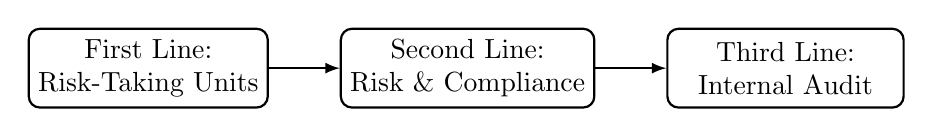
\begin{tikzpicture}[>=latex,thick,node distance=0.9cm]
        \node[draw,rounded corners,minimum width=3.0cm,minimum height=1.0cm,align=center] (first) {First Line:\\Risk-Taking Units};
        \node[draw,rounded corners,minimum width=3.0cm,minimum height=1.0cm,right=of first,align=center] (second) {Second Line:\\Risk \& Compliance};
        \node[draw,rounded corners,minimum width=3.0cm,minimum height=1.0cm,right=of second,align=center] (third) {Third Line:\\Internal Audit};
        \draw[->] (first) -- (second);
        \draw[->] (second) -- (third);
    \end{tikzpicture}
\end{lrbox}
\ifdim\wd\bookmeasuredbox<0.65\linewidth
\setlength{\bookcapwidth}{0.65\linewidth}
\else
\setlength{\bookcapwidth}{\wd\bookmeasuredbox}
\fi
\ffigbox[\bookcapwidth]{
\usebox{\bookmeasuredbox}
}{
    \caption{The three lines of defense in risk governance}
    \label{fig:three_lines}
}
\end{figure}

The first line of defense is the business unit that actually takes the risk, a trading desk or a lending team, and is responsible for managing it day to day within approved limits.
The second line is an independent risk management and compliance function, organizationally separate from the business units it oversees, that builds and maintains models like the VaR and economic capital methods introduced in this chapter and the credit-scoring methods of Chapter 9, sets risk limits, and monitors whether the first line is operating within them.
The third line, internal audit, periodically and independently verifies that the first two lines are functioning as intended, checking not just whether a number was computed correctly but whether the entire risk management process was followed. This structure exists specifically to prevent the single point of failure that arises when the people generating revenue from a risk position are also the people responsible for measuring and reporting that risk, a conflict of interest that has been implicated in numerous historical risk management failures.

A model like the ones developed in this chapter is only as trustworthy as the governance structure that surrounds it: a perfectly specified VaR model computed by a risk function with no real independence from the trading desk it monitors provides little genuine protection.
The second line of defense is typically led by a Chief Risk Officer (CRO), a senior executive with direct reporting access to the board of directors' risk committee, independent of the chief executive and business-line management, specifically so that a risk concern can reach the board without first being filtered by the same management chain whose performance the concern might reflect poorly on.
This reporting-line independence is not a bureaucratic formality. Several well-documented historical risk management failures trace back to a risk function that identified a genuine problem internally but lacked the organizational standing or independence to have that concern acted on before it caused a material loss. That is precisely why modern governance codes and regulatory guidance treat CRO independence, board-level risk reporting, and the second line's authority to veto or unwind a position as essential features of a credible risk management function rather than optional best practices.

A concrete limit example shows how these three lines actually interact day to day. Suppose the second line has approved a daily 99\% VaR limit of \$300,000 for the desk running the \$10 million portfolio from Table~\ref{tab:portfolio_returns}. The parametric $99\%$ VaR of \$250,081 computed in Section~\ref{sec:var} represents a limit utilization of $250{,}081/300{,}000 \approx 83.4\%$, comfortably within the approved limit, so the first line continues trading within its normal risk-taking mandate and the second line's monitoring is routine.
Now suppose realized volatility rises sharply enough, following the volatility-adjusted VaR logic of Section~\ref{sec:garch-var}, that the desk's VaR the next day increases to \$340,000, a breach of \$40,000, or roughly $13.3\%$ over the approved limit.
This is precisely the event the three-lines structure exists to catch. The breach must be reported to the second line the same day, which independently assesses whether the increase reflects a temporary, defensible spike in market volatility or a genuine change in the desk's risk profile that warrants an immediate position reduction. A limit breach that recurs or is not promptly remediated is the kind of finding the third line's periodic audit is designed to flag, even if the second line's day-to-day response was otherwise adequate.

\section{Case Vignette: When Value at Risk Meets a Genuine Crisis}

The 2008 financial crisis is the standard cautionary tale about the limits of the methods developed in this chapter, and it is worth walking through precisely why, since the failure was not a matter of arithmetic errors. Many large banks entered 2008 with VaR models built and validated exactly as this chapter describes: parametric or historical methods, calibrated on several years of historical returns, backtested against the kind of exception-counting procedure in Section~\ref{sec:backtesting-var}, and generally passing those backtests during the calm years leading up to the crisis.
Several major banks subsequently reported, in hindsight, that they experienced multiple trading days during the crisis with losses their models had classified as ``25-standard-deviation events,'' occurrences that a normal distribution assigns a probability of essentially zero, and that should therefore not occur even once across the entire history of the universe under the model's own assumptions, let alone several times in a single year.

This did not mean the underlying arithmetic was wrong; it meant the normality assumption, the same parametric assumption used throughout Section~\ref{sec:var} of this chapter, was a poor description of returns during a genuine crisis, the fat-tails caveat flagged repeatedly throughout this book. A model calibrated on a multi-year window that happened not to include a severe crisis will, by construction, underestimate the frequency of extreme moves, since it has literally never observed one in its training data, the same finite-sample problem behind this chapter's caution about short backtesting windows.
Compounding this, correlations between asset classes that had appeared low or stable during calm periods rose sharply during the crisis, a pattern sometimes summarized as ``correlations go to one in a crisis,'' which meant that diversification benefits assumed by portfolio-level VaR calculations, including the variance-covariance approach in Section~\ref{sec:matrix-var}, provided far less protection than historical correlations had suggested they would.

The lesson this vignette is meant to leave is not that VaR or Expected Shortfall are poor tools; both remain standard, required practice at every major financial institution today. It is that every method in this chapter answers the question it was designed to answer only as well as its underlying assumptions hold. A serious risk management practice therefore treats stress testing, backtesting, and the qualitative judgment of an independent second line of defense as necessary complements to any single statistical model, not optional extras.

The regulatory response to this episode is worth naming explicitly, since it shaped the risk management landscape this chapter describes.
The Basel Committee's Fundamental Review of the Trading Book (FRTB)\index{Fundamental Review of the Trading Book (FRTB)}, finalized in the years following the crisis and phased in at internationally active banks through the early 2020s, replaced VaR with Expected Shortfall as the basis for market-risk capital calculations. The reason is that ES, unlike VaR, is sensitive to the severity of losses beyond the threshold, not merely their frequency. That addresses the ``25-standard-deviation event'' problem described above directly: a VaR-based capital charge is blind to how much worse the tail beyond the VaR threshold actually is, while an ES-based charge is not.
FRTB also requires banks to calibrate their models using a period of significant historical stress, rather than only recent, potentially calm data, a direct regulatory response to the finite-sample, calm-period-calibration problem this vignette illustrates, and introduces a more granular desk-level model approval process so that a single bank-wide model validation can no longer mask weaknesses in how any one specific trading desk's risk is measured. None of this makes the statistical methods in this chapter obsolete; it makes them subject to a considerably more demanding, and more explicitly crisis-aware, regulatory standard than the pre-2008 VaR framework was.

\section{Challenges in Market Risk Management}

Several challenges recur across nearly every market risk management application, and Chapter 9 revisits several of them in a credit-risk setting.

\textbf{Model risk in the risk model itself.} Every method in this chapter, parametric VaR's normality assumption, the GARCH recursion's own parametric structure, the delta-normal method's linearity assumption, is itself a model with assumptions that can fail exactly when they matter most, during a crisis. A risk model that works well in calm markets can dramatically understate risk in a crisis precisely because crises are, by definition, unusual, low-probability events that a model calibrated on typical conditions was never designed to capture.
The gap between a linear approximation and a full, nonlinear revaluation, small for a modest move, can widen substantially exactly when the move being measured is largest.

\textbf{Correlation and tail dependence.} Individual risk measures often look reasonable in isolation, but a real portfolio becomes dangerous when many positions move together at the worst possible time, a pattern called tail dependence.
This chapter's own case vignette showed a concrete, historically documented instance: correlations that looked low and stable during calm markets rose sharply during the 2008 crisis, eroding the diversification benefit the variance-covariance VaR of Section~\ref{sec:matrix-var} assumed. Estimating tail dependence directly, rather than assuming a single, stable correlation matrix, is both statistically difficult and highly consequential for the resulting risk estimate.

\textbf{Procyclicality.} Risk measures calibrated on recent data tend to show low risk during calm periods (encouraging more risk-taking and leverage) and high risk immediately after a shock has already occurred (forcing deleveraging precisely when the system can least afford it), an amplifying feedback loop that has been implicated in several historical financial crises and that no purely statistical risk measure resolves on its own.

\textbf{Data quality and limited loss history.} Severe market crashes are, fortunately, rare, which means the historical data available to estimate their probability and severity is inherently limited, the small-sample problem flagged repeatedly throughout this book's time series and statistical inference material, and illustrated directly by this chapter's own twenty-observation VaR and backtesting examples. A VaR model estimated from a calm multi-year window that happened not to include a severe crisis will systematically understate tail risk.

\textbf{Regulatory and business tension.} Risk models exist within an organization that also wants to grow revenue and take on positions, and a risk function that is too conservative can be overridden or under-resourced, while one that is too permissive can miss a crisis entirely; getting this balance right is as much an organizational and governance challenge as a statistical one.

\textbf{Regulatory arbitrage.} Whenever regulatory capital is calculated from a bank's own reported VaR figure, as under the Basel backtesting multiplier described above, an institution has some incentive to structure its risk reporting specifically to minimize the resulting capital charge rather than its actual underlying risk. That might mean choosing a favorable historical window, a favorable confidence level, or a model specification that happens to backtest well. The resulting gap between measured and true risk can widen quietly over time, even when every individual calculation is technically correct.

\textbf{Limit-setting on a diversification-sensitive measure.} Component VaR's dependence on the full correlation structure of the book, not just an individual position's own volatility, cuts both ways. It correctly rewards genuinely diversifying positions with a smaller risk charge. But a desk operating close to its limit has some incentive to seek out positions that look diversifying under the currently estimated, calm-period correlation matrix, the positions Section~\ref{sec:stress-testing}'s correlation stress test warns can stop diversifying, and start actively compounding losses, the moment correlations move against the book during a genuine crisis.

\textbf{Machine learning adds a further layer of model risk.} As Chapter 6 discussed, a neural network or gradient-boosted model can, in principle, forecast volatility or tail risk more flexibly than GARCH or a simple historical window, capturing nonlinear patterns a fixed parametric form cannot. But it inherits that chapter's overfitting\index{overfitting} and interpretability concerns in a setting where the consequences of an undetected error are unusually severe. An opaque VaR model that a regulator or independent validator cannot fully interrogate is a much harder model to trust with a bank's reported capital requirement, regardless of its backtested accuracy.

\section{Key Takeaways}

Market risk management complements the prediction-focused methods of earlier chapters by asking how bad outcomes can get, not just what is expected to happen. Value at Risk and Expected Shortfall summarize the downside of a return distribution using parametric, historical, or Monte Carlo methods; each involves a real tradeoff between distributional assumptions and finite-sample noise, and Expected Shortfall is generally preferred to VaR precisely because it accounts for the severity of losses beyond the VaR threshold rather than only their frequency, even though backtesting that severity directly is a genuinely harder problem than counting VaR exceptions.

Volatility itself need not be treated as fixed: Chapter 7's GARCH model lets a VaR estimate update immediately after a large move, rather than waiting for a slow-moving historical average to catch up, filtered historical simulation combines that responsiveness with the historical method's distribution-free flexibility, and the delta-normal approximation, while a convenient linearization for options portfolios, understates risk in proportion to the gamma exposure it ignores, a gap a second-order delta-gamma correction closes almost entirely.

Component VaR carries this same portfolio-level thinking one step further, decomposing total risk into per-position contributions that depend on the whole book's correlation structure rather than any position's standalone volatility, which is why a stress test that pushes correlations toward the crisis-period pattern this chapter's case vignette describes can more than double measured portfolio risk without any individual position's own volatility changing at all.

No aggregate should ever be the only thing anyone looks at. Sensitivities sit alongside VaR rather than beneath it, because a single portfolio-level number necessarily discards the information about \emph{where} the risk is: a rate book can report a net DV01 of exactly zero while carrying a \$1.36 million exposure to a curve flattening, and an options position's VaR can be computed correctly to the cent while remaining structurally blind to a routine move in implied volatility. Producing those sensitivities at the scale a real book requires is itself solved by reverse-mode automatic differentiation, the identical algorithm that trains neural networks.

Measurement is also not the same thing as management. Hedging exchanges an unwanted exposure for a smaller, differently-shaped residual rather than eliminating risk; position sizing controls risk before it is taken, which makes it only as good as the volatility forecast behind it; and stop-losses, the crudest control of the three, are lagging by construction and rescue far less of a drawdown than intuition suggests. None of these methods is self-policing either: backtesting (including Basel's own traffic-light zones), independent model validation, and a governance structure like the three lines of defense are what actually catch a miscalibrated model before it causes a loss, rather than after.

Across every method in this chapter, the central lesson is the same one that closed Chapter 5's discussion of valuation: a risk number is only as trustworthy as the assumptions behind it, and a serious risk management practice combines several methods, and an honest accounting of where they disagree, rather than relying on any single measure alone. Chapter 9 now turns to the analogous toolkit for credit risk.

\section{Suggested Exercises}

\begin{enumerate}
    \item Explain, in your own words, the difference between Value at Risk and Expected Shortfall, and describe a situation in which two portfolios could have identical VaR but very different Expected Shortfall.
    \item Using the returns in Table~\ref{tab:portfolio_returns}, compute the parametric 90\% VaR (using $z_{0.90}=1.282$) for the \$10 million portfolio, and compare it to the 95\% and 99\% figures computed in the chapter.
    \item Using the historical method, compute the 90\% VaR and Expected Shortfall from Table~\ref{tab:portfolio_returns} (the 90\% VaR corresponds to the second-worst return out of twenty observations).
    \item Using Table~\ref{tab:portfolio_returns}'s cumulative value path and the definition in Section~\ref{sec:max-drawdown}, compute the drawdown at Day 6 (relative to the running peak established by that point) and compare it to the chapter's maximum drawdown of $6.74\%$, realized only at Day 20. Explain why a portfolio can pass through a large intermediate drawdown that is later exceeded by an even larger one, rather than the path recovering.
    \item Using Chapter 7's GARCH(1,1) recursion values at $t=2$ ($\sigma=2.03\%$) and $t=5$ ($\sigma=1.99\%$), compute the parametric 95\% VaR of a \$5 million position at each date, and explain why the two figures are so much closer together than the $t=3$-versus-$t=4$ comparison in the text.
    \item Explain why a portfolio's 99\% VaR can be smaller than its loss under a stress-test scenario, and why this is not evidence that the VaR calculation is wrong.
    \item A bank's VaR model produces 7 exceptions over a rolling 250-day window at the 99\% confidence level. Using the Basel traffic-light framework, classify this outcome and explain what supervisory consequence it would typically trigger.
    \item Using the delta-normal example in Section~\ref{sec:delta-normal}, recompute the 95\% and 99\% delta-normal and full-revaluation VaR for a position that is instead \emph{long} 1,000 calls, and explain which direction of stock-price move now represents the position's worst case.
    \item Pick two of the challenges listed in this chapter and describe a concrete scenario, not already used in the text, in which that challenge could cause a risk management system to understate a firm's true risk.
    \item Using Section~\ref{sec:matrix-var}'s two-asset covariance matrix, recompute the portfolio's volatility and 95\% VaR under a stressed correlation of $\rho=0.8$ instead of the $\rho=0.5$ used in the text, and compare the resulting increase to the one computed in Section~\ref{sec:stress-testing}.
    \item A bank has \$60 million in high-quality liquid assets and projected net cash outflows of \$55 million over a 30-day stress scenario. Compute its LCR, and explain why a bank could satisfy the LCR comfortably while still having an inadequate NSFR.
    \item A third asset, AssetC, is added to Section~\ref{sec:matrix-var}'s two-asset position with a Component VaR of \$4,000. Using the fact that Component VaRs must sum to the portfolio total, explain what this implies about how AssetC is correlated with the existing AssetA/AssetB position, without needing to know AssetC's own standalone volatility.
    \item Using this chapter's three-lines-of-defense limit example, compute the limit utilization if the approved daily VaR limit were instead \$275,000 (holding the parametric 99\% VaR of \$250,081 fixed), and explain whether a subsequent rise in VaR to \$290,000 would count as a limit breach under this tighter limit.
    \item Using this chapter's reverse-stress-testing example, compute the single-day return that would exhaust a risk capital cushion of \$800,000 instead of \$500,000 for the same \$10 million portfolio, and explain whether the $-7\%$ historical stress scenario from Section~\ref{sec:stress-testing} would still exceed this larger cushion.
    \item Explain, using this chapter's FRTB discussion, why a capital framework based on Expected Shortfall is less vulnerable than a VaR-based framework to a repeat of the ``25-standard-deviation event'' problem described in the 2008 case vignette.
    \item Using Section~\ref{sec:econ-capital}'s square-root-of-time rule, compute the 5-day regulatory VaR implied by the parametric 99\% VaR of \$250,081, and explain why this figure is smaller than the 10-day figure computed in the chapter even though both are scaled from the same 1-day VaR.
    \item Section~\ref{sec:econ-capital} showed that a modest positive autocorrelation of $\phi=0.10$ makes the square-root-of-time rule understate 10-day VaR by about $9.4\%$. Explain, in your own words, why a \emph{negative} autocorrelation (mean reversion) in daily returns would instead make the square-root-of-time rule \emph{overstate} multi-day risk, and describe a market condition in which returns might plausibly exhibit this pattern.
    \item Using the vega in Table~\ref{tab:greek_limits}, compute the profit or loss on the short 1,000-call position if implied volatility rises by three percentage points while the stock price does not move at all, and express it as a percentage of the position's $95\%$ full-revaluation VaR of \$980.79 from Section~\ref{sec:delta-normal}. Explain why no amount of backtesting the VaR model would have revealed this exposure.
    \item Apply a \emph{steepening} scenario to the DV01 ladder of Table~\ref{tab:dv01_ladder}, in which two-year yields fall 10 basis points, five-year yields fall 5, ten-year yields rise 10, and thirty-year yields rise 15. Compute the desk's profit or loss, and explain why the sign of the result is the opposite of the flattening scenario worked in the text even though the net DV01 is zero in both cases.
    \item A trading book is exposed to 500 distinct risk factors. (a) How many full valuations are required to produce a complete set of first-order sensitivities by bump-and-revalue? (b) Roughly how many are required by adjoint algorithmic differentiation, and why does this figure not depend on the number 500? (c) Explain why gamma, unlike delta, is not obtained for free in the same reverse sweep, and name the machine learning computation that faces the same first-order-versus-second-order cost distinction.
    \item Using Section~\ref{sec:managing-risk}'s volatility-targeting calculation, recompute the dollar amount to hold in the risky portfolio (a) if the mandate's target volatility were $15\%$ rather than $10\%$, and (b) if the daily volatility estimate were instead Chapter 7's GARCH post-shock forecast of $2.08\%$, holding the $10\%$ target. Comment on the size of the position change in (b) and on what it implies about how often a volatility-targeted portfolio must trade.
    \item Show that the residual loss on a delta-hedged short-gamma position grows quadratically, by recomputing Section~\ref{sec:managing-risk}'s figure of \$61.72 for a stock move twice as large as the \$2.198 used there. Explain why the residual is a loss for \emph{both} a rise and a fall in the stock price, and what this implies about the kind of bet a delta-hedged option seller is really making.
    \item \textbf{Challenge (real data).} Download at least two years of daily prices for a small portfolio of real stocks (for example, three to five components of a major index, via \texttt{yfinance}) and compute the portfolio's daily returns using fixed weights of your choosing. (a) Compute the portfolio's parametric and historical $99\%$ one-day VaR, as in Section~\ref{sec:var}, and compare the two estimates. (b) Backtest your parametric VaR estimate over the full sample using Kupiec's test, referenced in Section~\ref{sec:backtesting-var}: count the number of days on which the realized loss exceeded the VaR estimate, and determine whether the exception rate falls inside the Basel traffic-light green zone for your sample size. (c) Real portfolio returns are typically both fat-tailed and volatility-clustered, unlike the twenty-observation toy example this chapter builds on; discuss whether your backtest results suggest the parametric (normal-distribution) VaR model over- or understates risk relative to the historical method, and connect this to this chapter's own discussion of GARCH-based, volatility-adjusted VaR.
\end{enumerate}

\section{Further Reading}

\begin{itemize}
    \item Jorion, \emph{Value at Risk: The New Benchmark for Managing Financial Risk}. The standard reference for VaR methodology, covering the parametric, historical, and Monte Carlo approaches introduced in this chapter in much greater depth and rigor.
    \item Hull, \emph{Risk Management and Financial Institutions}. A broad treatment of market, credit, and operational risk within financial institutions, extending this chapter's introductory coverage of each risk type.
    \item McNeil, Frey, and Embrechts, \emph{Quantitative Risk Management}. A mathematically rigorous treatment of coherent risk measures, Expected Shortfall, and the tail-dependence and correlation issues raised in this chapter's challenges section.
    \item Basel Committee on Banking Supervision, \emph{Basel III: A Global Regulatory Framework for More Resilient Banks and Banking Systems}. The primary regulatory source for the capital adequacy, backtesting, and liquidity-coverage concepts introduced in this chapter. Its market-risk successor, \emph{Minimum Capital Requirements for Market Risk} (January 2016, rev.\ February 2019), is the standard produced by the Fundamental Review of the Trading Book: it replaced Value at Risk with Expected Shortfall as the regulatory measure and introduced the sensitivities-based capital charge that this chapter's treatment of sensitivity-based risk limits develops.
    \item Giles, M.\ and P.\ Glasserman, ``Smoking Adjoints: Fast Monte Carlo Greeks,'' \emph{Risk}, January 2006. The paper that introduced adjoint differentiation to derivatives risk management, and the direct source for Section~\ref{sec:aad}'s claim that a full set of sensitivities costs a small constant multiple of a single valuation.
    \item Baydin, A.\ G., B.\ A.\ Pearlmutter, A.\ A.\ Radul, and J.\ M.\ Siskind, ``Automatic Differentiation in Machine Learning: A Survey,'' \emph{Journal of Machine Learning Research}, vol.\ 18, 2018. A clear and self-contained account of forward- and reverse-mode automatic differentiation, written for the machine learning audience, making explicit the equivalence with backpropagation that Section~\ref{sec:aad} relies on.
    \item Crouhy, Galai, and Mark, \emph{The Essentials of Risk Management}. A practitioner-oriented synthesis spanning market, credit, and operational risk, model validation, and risk governance, tying together the full breadth of topics covered in this chapter and Chapter 9 in a single volume.
\end{itemize}

\end{document}

